\documentclass{sigcomm-alternate}

\usepackage[utf8x]{inputenc}
\usepackage[hyphens]{url}
\usepackage{hyperref}

%\usepackage[longnamesfirst,sort,square]{natbib}


\begin{document} 
\title{Who Turned off the Internet?} 
\subtitle{Mining Temporary Unreachability\\ \Large Intermediate Report }

\numberofauthors{1} 
\author{ \alignauthor Daniel Aschwanden\\
%\affaddr{Communication Systems Group}\\
%\affaddr{Institute TIK}\\
\affaddr{ETH Zurich}\\
\email{asdaniel@ee.ethz.ch}\\
}

\maketitle 
%%%%%%%%%%%%%%%%%%%%%%%%%%%%%%%%%%%%%%%%%%%%%%%%%%%%%%%%%%%%%%%%
\section{Introduction}
The end-to-end connectivity of hosts is the key service of the Internet.
However, even after 40 years of intense engineering efforts, this
connectivity is temporally broken for various reasons, such as link
or hardware failure \cite{Markopoulou:2008}, mis-configurations
\cite{Mahajan:2002}, or natural disasters
\cite{Dainotti:2012:EBH,Schulman:2011}.
This shows that there is a real need for methods to systematically
detect and locate Internet outages of remote autonomous systems,
subnets, and even single hosts. An automated, ongoing detection and
tracking of connectivity issues of the Internet is particularly
interesting for Internet Service Providers as it may generate
transparent outage information for customers and enables the ISP
to react adequately on detected reachability problems and prevent
expensive debugging sessions.

Researchers and industrial vendors have proposed various approaches
for systematically detect, locate and troubleshoot Internet outages
and loss of end-to-end reachability.

Basically, reachability can be assessed from two perspectives:
data-plane and control-plane measurements. By using control-plane
information, most researchers focussed on approaches detecting
problem related to address space, i.e. bogon advertisements
\cite{Feamster:2005}, prefix hijacking \cite{Zhang:2010},
or BGP misconfiguration \cite{Mahajan:2002}. Bush et
al.\cite{Bush:Optometry} pointed out, that tracking data-plane
reachability with control-plane information such as BGP is heavily
inaccurate due to the effect of secret peering policies, i.e. default
routes which allows packets to reach their destination even when a
corresponding route is missing.
Moreover, connectivity issues imposed by packet filtering cannot
be tracked by control-plane approaches \cite{Dainotti:2011:ACI}.

To sum up, control-plane measurements of reachability are indirect
and thus of limited practical usage for systematical reachability
tracking.

In contrast, measurements of the data-plane are direct and can be
more accurate regarding end-to-end reachability. Data-plane
measurements can be divided into active probes and passive monitoring.
Whereas active probes generates additional traffic towards the
observed address space of the Internet, passive monitoring relies
fully on the traffic generated by servers and clients of the network.

Active probing is widely used for end-to-end reachability problem
detection, ranging from rudimentary debugging tools as ping
\cite{PING}, paris traceroute \cite{traceroute} or nmap \cite{Nmap}
to highly sophisticated, automated outage detection tools as Hubble
\cite{Katz:2008} or PlanetSeer \cite{Zhang:2004}. \cite{Bush:Optometry}
pointed out there exist some important limitations as packet filtering
by firewall and NAT devices or suboptimal routing which result in
intermittent problems as packet rerouting. Furthermore, there is
no active probing technique known which is able to record the return
path in addition to the forward-path. It is not generally true to
deduce that forward-path reachability implies return-path reachability
as well, since there may be intermittent problems caused by suboptimal
routing \cite{Bush:Optometry}. Furthermore, the emerging usage of IPv6
addresses imposes an additional challenge regarding the scalability of
all these active probing. Quan et al.\cite{Quan12a} proposed an approach
which

To fill this gap, \cite{SchatzmannPAM2011} proposed the fully
passive approach called FACT relying on flow level information to
identify remote connectivity problems. The basic idea of FACT is to
match the corresponding outgoing and incoming flow to a bidirectional
connection. Then the remaining unidirectional connections or unresponsive
connections are extracted and investigated. The detection of an outage
is consolidated by aggregating these unresponsive connections to host,
network and AS level and rating the severity of the events by affected
users. This consolidation is required to reduce the noise of unresponsive
connections caused for example by scanning or botnets and implies an
implicit prioritization of events which affect many internal network
users.

To further improve the reporting functionalities of FACT Schatzmann et
al. proposed in \cite{MyPhDThesis} to treat certain types of Internet
services differently that don't require constant reachability.
For example, Skype or Bitrorrent applications that are executed on
client machines such as Destops, Laptops, or Smartphons are possible
only reachable for limited time during a day. This characteristic is
caused by the fact that these machines are often disconnected from the
network to save power or due to user mobility effects. However, this
temporal unreachability is not noted as a problem by the end-users.
Therefore this issues should be tagged by FACT with a low severity (low
priority for the operator). To achieve this Schatzmann et al. presented
in \cite{MyPhDThesis} a hybrid service classification system to label
the type service such as http, skype, or bittorrent provided by host
requiring only limited processing and collection efforts.

In this work, we plan to enrich the reporting functionalities of FACT
with a other key aspect, namely the knowledge about the past stability,
popularity characteristics of remote sites. In more detail, we plan to
analyses the stability, popularity characteristics of remote sites over
longer time scales and use this information within FACT to further
improve the prioritization of connectivity issues.  As example, a
remote web server used only by a few users that is often unreachable
(overloaded, used for testing?) should not have the same weight within
the prioritization algorithm of FACT like a popular content distribution
host that was always reachable over the past.

%However, the drawback of this aggregation is that the approach is too
%coarse grained to track service outages which may be also important,
%especially if they are important services.

%Furthermore, FACT's outage detection is solely based on traffic to
%TCP port 80 in the hope that the process listening to port 80 is a
%stable service, e.g. a web server. Since TCP traffic to port 80 is
%sometimes used by various application protocols different than HTTP,
%e.g. Skype, to traverse firewall and NAT devices, this assumption is
%not true in general. Depending on the kind of service or application,
%the characteristics of its stability and uptime differ significantly,
%i.e. if a host is a web server providing important content which should
%be up most of the time, or in the case of a Skype super-node, which is
%systematically changing over time. However, from a flow perspective the
%connections to a Skype super-node or to a web server look very similar
%and are often indistinguishable.
%
%For this reason, the services behind the traffic which FACT is using
%for outage detection have to be monitored on a longer time scale and
%characterized by its stability, relevance and popularity. Afterwards,
%from these characterized services a smart selection of stable and
%representative targets is created and fed into FACT for tracking remote
%connectivity issues. To this end, the observed traffic used for the
%outage detection can be generalized such that not only traffic to TCP
%port 80 is considered anymore.
%
To sum up, the overall goal of this thesis is to extend FACT with
a service monitoring and classification functionality to employ a
third level of noise reduction besides user aggregation and traffic
preselection. In fact, this functionality should enable FACT to focus
even better relevant connectivity issues which are related to a stable
and popular service.

\section{Approach}
To achive this goal to enrich the reporting functionalities of FACT
with knowledge about the past stability, popularity characteristics 
of remote sites we plan to extent FACT by using three stpes as 
illustrated in Figure X

\begin{figure*}[ht!]
\centering 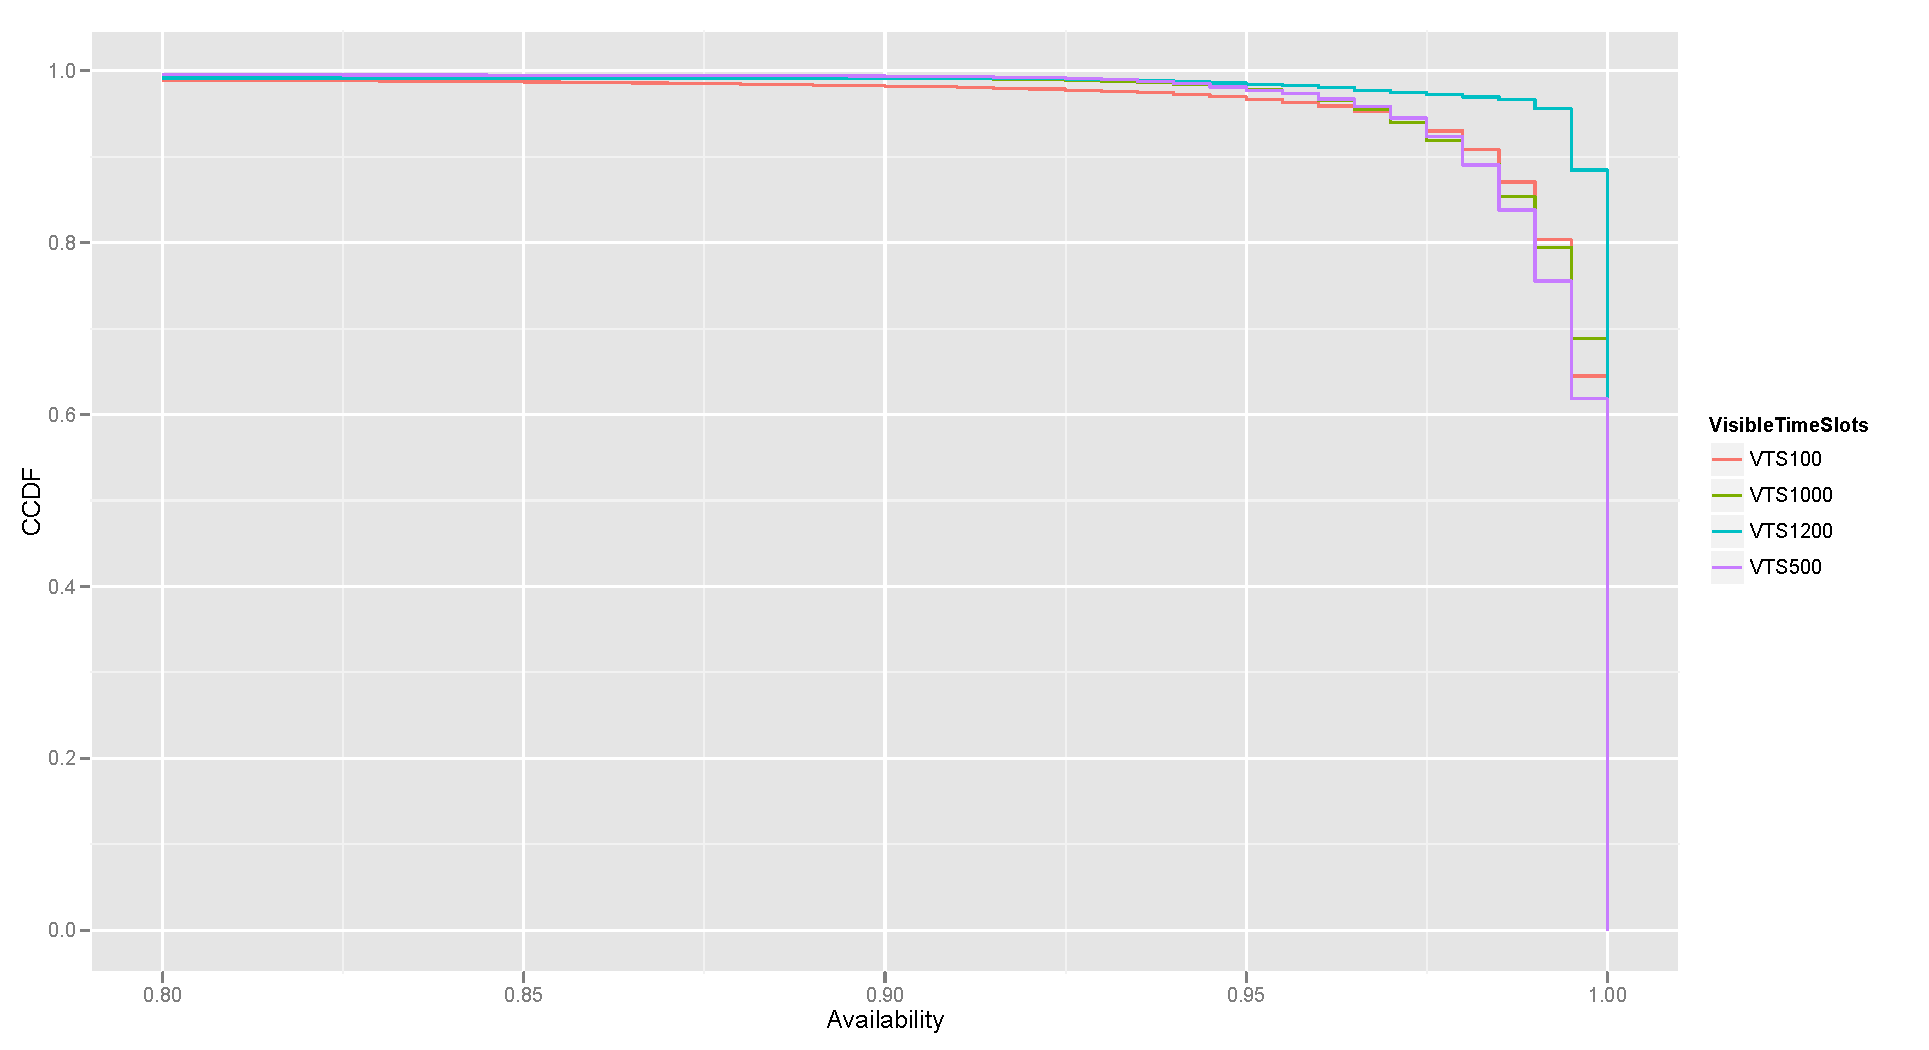
\includegraphics[width=18cm]{images/RATIO_VTS_External.pdf}
\caption{CCDF of availability with respect to visibility}
\label{fig:RatioVTS} 
\end{figure*}


%In a first step, the server socket detection is implemented. The
%challenge of the server socket detection lies in the fact that the
%netflow data does not provide enough precise timing information to
%determine which flow is originated from the client and thus determine
%the server's socket. Therefore, the server socket detection is
%achieved by the assumption that server sockets act as concentrators
%in the sensei that several clients have connections to the identical
%server socket.

a first step,  server socket detection is implemented. The
challenge of the server socket detection lies in the fact that the
netflow data does not provide enough precise timing information to
determine which flow is originated from the client and thus determine
the server's socket. Therefore, the server socket detection is
achieved by the assumption that server sockets act as concentrators
in the sensei that several clients have connections to the identical
server socket.

Secondly, the previously detected server sockets are continually
monitored and especially the successful and unsuccessful connection
attempts are recorded. Furthermore, these information are used to update
the statistical information of visibility, popularity and stability.

In a third step, the number of server sockets have to be reduced and
selected in a smart way such that FACT is able to use these sockets
for outage tracking. In particular, the server sockets coverage of the
Internet address space has to be optimized. It makes no sense to select
only the most popular sockets if they are all located in the same /24
network.

Finally, FACT has to be adopted to optimally use the preselected server
sockets for tracking only relevant connectivity issues by reducing
network outage alerts based on single host outages of unstable services.

\section{Preliminary Results} \begin{figure*}[ht!]
\centering 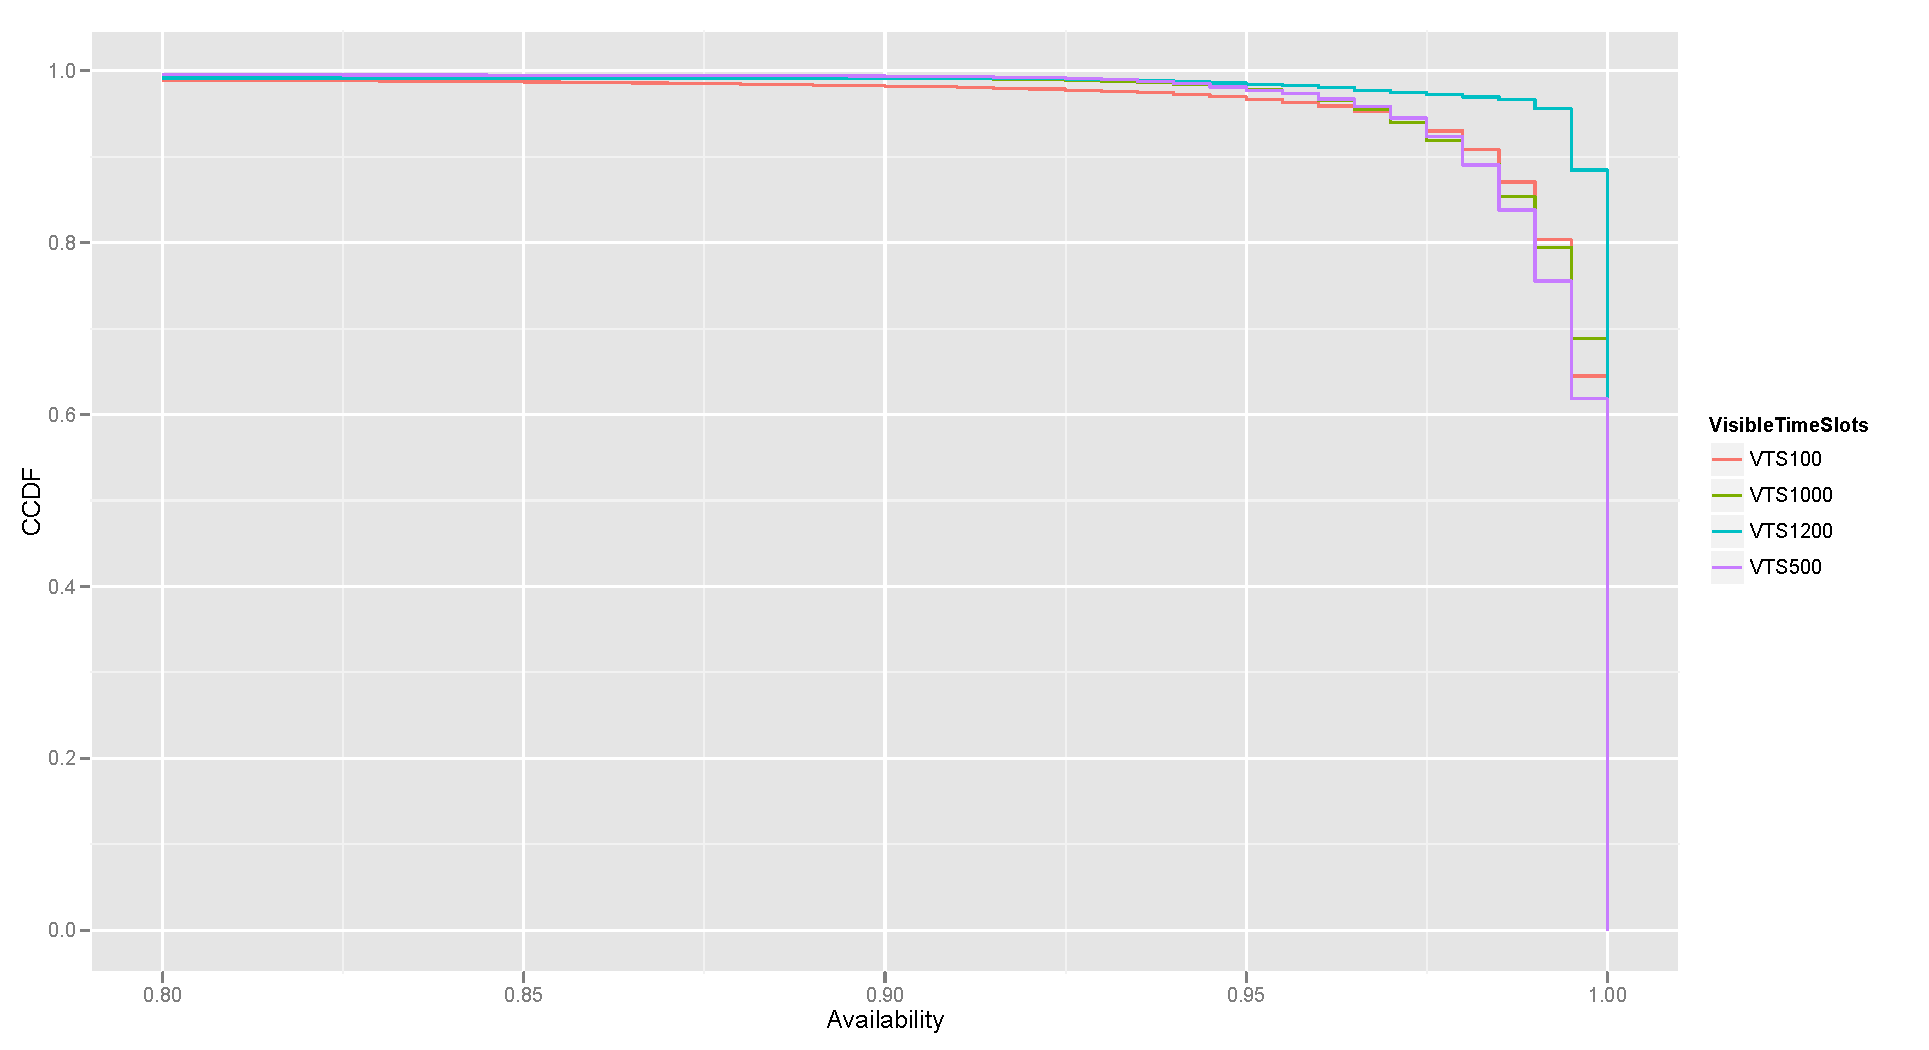
\includegraphics[width=18cm]{images/RATIO_VTS_External.pdf}
\caption{CCDF of availability with respect to visibility}
\label{fig:RatioVTS} \end{figure*} The server socket detection and
the ongoing monitoring thereof are already implemented. A one-week
long netflow data trace of november 2010 was used to test this
implementation.

Figure \ref{fig:RatioVTS} shows a complementary cumulative distribution
function of the availability of server sockets with respect to their
visibility. Intuitively, the server sockets which are almost always
contacted by internal network users should have a high availability,
i.e. important web servers or DNS servers. As it can be seen in
figure \ref{fig:RatioVTS} the curve "VTS1200", representing the
sockets which are contacted in more than $99\%$ of all 5 minute
long observation slots, yields a higher share on hosts with an
availability higher than $99.5\%$. This finding is the foundation
for this approach to track connectivity outages of important hosts.

Despite the fact that the "VTS1200" set contains only around $0.2\%$
of all known sockets of this observation week, they are still around
5000 distinct sockets.

Moreover, the Internet address space coverage of these almost always
visible sockets has to be carefully reviewed.

To sum up, the results of the preliminary analysis of this one week
long data trace deduce that the chosen approach is promising with
respect to noise reduction of FACT and to enhance FACT's reliability
on single host outages.

\bibliographystyle{abbrv} %\bibliographystyle{apalike}
\bibliography{95_bib} \end{document}
